% CVPR 2026 Paper Template (cvpr-org/author-kit, main branch of 2026-05-27; no CVPR 2027 kit had been released when this
% draft was started). Build: latexmk -pdf main.tex

\documentclass[10pt,twocolumn,letterpaper]{article}

%%%%%%%%% PAPER TYPE  - PLEASE UPDATE FOR FINAL VERSION
% \usepackage{cvpr}              % To produce the CAMERA-READY version
\usepackage[review]{cvpr}      % To produce the REVIEW version
% \usepackage[pagenumbers]{cvpr} % To force page numbers, e.g. for an arXiv version

% Import additional packages in the preamble file, before hyperref
%% This file contains a number of tweaks that are typically applied to the main document.
%% They are not enabled by default, but can be enabled by uncommenting the relevant lines.


%%
%% Official support for 2-column teaser figure
%%
\usepackage{cuted} %< for strip environment

%%
%% For auto-referencing of figures (see fig/teaser.tex and \label{} therein) 
%%
\usepackage{currfile} %< for \currfilebase macro

%%
%% caption and (global) spacing overrides
%%
\usepackage{caption} %< for "\captionof" commands (teaser)
% \setlength{\abovecaptionskip}{.5em} % space above caption
% \setlength{\belowcaptionskip}{1em} % space below caption

%%
%% Inline annotations; for predefined colors, refer to "dvipsnames" in the xcolor package:
%% https://tinyurl.com/overleaf-colors
%%
\newcommand{\red}[1]{{\color{red}#1}}
\newcommand{\todo}[1]{{\color{red}#1}}
\newcommand{\TODO}[1]{\textbf{\color{red}[TODO: #1]}}
%%
%% Disable for camera ready / submission by uncommenting these lines:
%%
% \renewcommand{\TODO}[1]{}
% \renewcommand{\todo}[1]{#1}

%%
%% Work harder in optimizing text layout. Typically shrinks text by 1/6 of page, enable
%% it at the very end of the writing process, when you are just above the page limit.
%%
% \usepackage{microtype}

%%
%% Fine-tune paragraph spacing.
%%
% \renewcommand{\paragraph}[1]{\vspace{.5em}\noindent\textbf{#1.}}

%%
%% Globally adjusts space between figure and caption.
%%
% \setlength{\abovecaptionskip}{.5em}

%%
%% Allows "the use of \paper to refer to the project name"
%% with automatic management of space at the end of the word.
%%
% \usepackage{xspace}
% \newcommand{\paper}{ProjectName\xspace}

%%
%% Commonly used math definitions.
%%
% \DeclareMathOperator*{\argmin}{arg\,min}
% \DeclareMathOperator*{\argmax}{arg\,max}

%%
%% Tighten underline.
%%
% \usepackage{soul}
% \setuldepth{foobar}

%%
%% Reconfigure paragraph (tweaks spacing)
%%

%%
%% Packages used by this paper
%%
\usepackage{graphicx}
\usepackage{booktabs}
\usepackage{multirow}
\usepackage{amsmath,amssymb}
\usepackage{xspace}
\usepackage{makecell}
\newcommand{\pizf}{$\pi_{0.5}$\xspace}
\newcommand{\ours}{DCS\xspace}   % decision-time counterfactual supervision
\newcommand{\ect}{ECT\xspace}
\newcommand{\pt}{\textsc{3D-Point}\xspace}
\newcommand{\pending}[1]{\textcolor{orange}{#1}}  % numbers still running; remove before submission
\usepackage{pgfplots}
\pgfplotsset{compat=1.17}
\usepgfplotslibrary{groupplots}
% categorical slots (validated: lightness, chroma, CVD and normal-vision separation; slot 3 below 3:1 contrast,
% so its bars carry direct value labels)
\definecolor{seriesA}{HTML}{2A78D6}  % pi0.5
\definecolor{seriesB}{HTML}{EB6834}  % ECT
\definecolor{seriesC}{HTML}{1BAF7A}  % DCS (ours)
\definecolor{inkMuted}{HTML}{52514E}


\definecolor{cvprblue}{rgb}{0.21,0.49,0.74}
\usepackage[pagebackref,breaklinks,colorlinks,allcolors=cvprblue]{hyperref}

%%%%%%%%% PAPER ID  - PLEASE UPDATE
\def\paperID{*****} % *** Enter the Paper ID here
\def\confName{CVPR}
\def\confYear{2026}

%%%%%%%%% TITLE
\title{Knowing Where, Not Going There:\\Vision-Language-Action Policies Encode Displacements They Do Not Act On}

%%%%%%%%% AUTHORS - anonymous for review
\author{Anonymous Authors\\
Anonymous Institution\\
}

\begin{document}
\maketitle
\begin{strip}
\centering
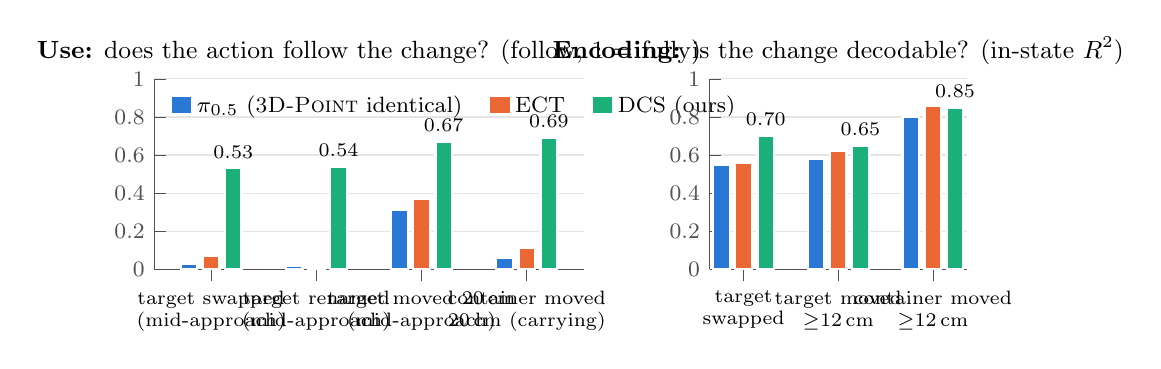
\begin{tikzpicture}
\begin{groupplot}[
    group style={group size=2 by 1, horizontal sep=1.6cm},
    ybar, /pgf/bar width=6pt, ymin=0, ymax=1.0, height=4.0cm,
    axis lines*=left, axis line style={inkMuted},
    tick style={inkMuted}, ticklabel style={font=\footnotesize, text=inkMuted},
    ymajorgrids, grid style={black!10},
    enlarge x limits=0.18,
    xtick=data, x tick label style={font=\footnotesize, align=center, text=black},
    every node near coord/.append style={font=\scriptsize, text=black},
    nodes near coords style={/pgf/number format/.cd, fixed, precision=2, zerofill},
    x tick label style={font=\scriptsize, align=center, text=black},
    title style={font=\small, yshift=-1ex},
  ]
  \nextgroupplot[
    width=0.58\textwidth,
    title={\textbf{Use:} does the action follow the change? (follow, 1 = fully)},
    symbolic x coords={swap,rename,moved,container},
    xticklabels={{target swapped\\(mid-approach)},{target renamed\\(mid-approach)},{target moved 20\,cm\\(mid-approach)},{container moved\\20\,cm (carrying)}},
    legend style={at={(0.02,0.97)}, anchor=north west, legend columns=3, draw=none, fill=none, font=\footnotesize,
                  /tikz/every even column/.append style={column sep=8pt}},
    legend image code/.code={\draw[#1, draw=none] (0cm,-0.08cm) rectangle (0.25cm,0.12cm);},
  ]
  \addplot[fill=seriesA, draw=white, line width=0.8pt] coordinates {(swap,0.03) (rename,0.02) (moved,0.31) (container,0.06)};
  \addplot[fill=seriesB, draw=white, line width=0.8pt] coordinates {(swap,0.07) (rename,0.01) (moved,0.37) (container,0.11)};
  \addplot[fill=seriesC, draw=white, line width=0.8pt, nodes near coords, nodes near coords align={vertical}]
    coordinates {(swap,0.53) (rename,0.54) (moved,0.67) (container,0.69)};
  \legend{{$\pi_{0.5}$ (\textsc{3D-Point} identical)},{ECT},{DCS (ours)}}
  \nextgroupplot[
    width=0.40\textwidth,
    title={\textbf{Encoding:} is the change decodable? (in-state $R^2$)},
    symbolic x coords={swap,target,container},
    xticklabels={{target\\swapped},{target moved\\$\geq$12\,cm},{container moved\\$\geq$12\,cm}},
  ]
  \addplot[fill=seriesA, draw=white, line width=0.8pt] coordinates {(swap,0.55) (target,0.58) (container,0.80)};
  \addplot[fill=seriesB, draw=white, line width=0.8pt] coordinates {(swap,0.56) (target,0.62) (container,0.86)};
  \addplot[fill=seriesC, draw=white, line width=0.8pt, nodes near coords, nodes near coords align={vertical}]
    coordinates {(swap,0.70) (target,0.65) (container,0.85)};
\end{groupplot}
\end{tikzpicture}
\captionsetup{hypcap=false}
\captionof{figure}{\textbf{\pizf knows where, but does not go there.} Probes at decision states of LIBERO-Object
rollouts (\cref{sec:probing}). \emph{Right:} the displacement of the target or the container is decodable from the action
tokens of every model. \emph{Left:} at the moments that decide the task, the action of \pizf barely follows it; neither
equivariant counterfactual training (\ect) nor an injected oracle 3D goal point (\pt, identical to \pizf) changes that.
Decision-time counterfactual supervision (\ours) does, without changing the encoding.}
\captionsetup{hypcap=true}
\label{fig:teaser}
\end{strip}

\begin{abstract}
Vision-language-action (VLA) policies that are near-perfect on LIBERO collapse once the objects in the scene trade
places: \pizf completes 99\% of LIBERO-Object episodes but only 19\% after two objects are swapped, driving to where the
target used to be.
We ask whether this is a failure of \emph{perception} or of \emph{use}.
Intervening on the simulator at arbitrary states of the policy's own rollouts, we measure, phase by phase, how far the
predicted action follows a displacement of the target or the container (use) and how well that displacement can be
decoded from the policy's hidden states (encoding).
\pizf encodes the displacement (in-state probe $R^2$ 0.55--0.86), yet at the moments the task is decided its action
follows it by only 3--22\%.
Two recent remedies leave use unchanged in a matched setting: equivariant counterfactual training on transformed
demonstrations, and injecting a privileged 3D goal point into the action expert, which is learned as a constant bias.
Supervising the policy in counterfactual worlds built at its own decision states, with privileged labels gated for
validity, raises use to 0.44--0.69 while encoding stays where it was.
Restricting which parameters may change localizes the effect: adapting only the VLM backbone, mostly its layers 9--17,
recovers about 90\% of the gain, whereas the action expert, its readout, or the VLM's keys and values alone do not.
Under the same teacher and training budget, this improves LIBERO-PRO object swaps by 30.8 points on LIBERO-Object and
14.3 points on LIBERO-Spatial over equivariant counterfactual training, at unchanged nominal success.
We also report what it costs: a trade-off with appearance changes, and a sensitivity to the furniture placement that
LIBERO re-draws at every reset, an evaluation detail we show moves per-task success by up to 25 points.
\end{abstract}

\section{Introduction}
\label{sec:intro}

Generalist vision-language-action (VLA) policies~\cite{brohan2023rt2,kim2024openvla,black2024pi0,pi2025pi05} now solve
the standard LIBERO suites~\cite{liu2023libero} almost perfectly.
The same policies fail in a strikingly simple way when the scene is rearranged.
The \emph{swap} perturbation of LIBERO-PRO~\cite{zhou2025liberopro} keeps every task and only lets the target trade places
with another object; under it, \pizf drops from 99\% to 19\% on LIBERO-Object and from 97.5\% to 40\% on LIBERO-Spatial.
Watching the rollouts shows why: the arm drives to where the target used to be.
The policy behaves as if the instruction retrieved a memorized trajectory~\cite{chen2026ect}.

A natural reading is that the policy does not \emph{perceive} where things are, and a large body of work adds
perception: depth, point clouds, 3D features, or an explicit 3D goal point~\cite{zhen20243dvla,qu2025spatialvla,tsai2026point}.
We test this reading directly and find it wrong for \pizf.
Because our policies run in a simulator, we can stop any rollout at any state, change exactly one thing (move the target,
swap it with another object, move the container while the object is carried, rename the target in the instruction),
re-render, and ask the policy again.
Comparing the two predictions measures how much the action \emph{uses} the change; probing the hidden states before and
after the change measures how well the change is \emph{encoded}.
The two disagree (\cref{fig:teaser}).
The displacement is linearly decodable from the action tokens of \pizf ($R^2$ 0.55--0.86), but at the moments that decide
the task, when the hand is still on its way to the target or carries the object to the container, the predicted action
follows the displacement by only 2--25\%.
\pizf \emph{knows where} the target is and does not \emph{go there}.

This distinction predicts which remedies can work, and \cref{sec:theory} makes the prediction precise: on fixed layouts
the data cannot tell a policy that uses the target's position from one that replays the memorized one.
If the information is already present, adding more of it should not help, and it does not: re-implementing the injection
of a privileged 3D goal point into the action expert~\cite{tsai2026point} in our setting leaves swap success at the base
level, and the injected channel is learned as a constant offset that ignores the point.
Equivariant counterfactual training (\ect)~\cite{chen2026ect}, which pairs demonstrations with geometrically transformed
replays, diagnoses the same memorization but, in a matched setting, leaves the measured use where it was.
What does change use is supervision \emph{at the decision states themselves}: building, at a state of the policy's own
rollout, a world in which the memorized action is wrong (the target or the container has moved) and supervising the
correct action there.
We call this decision-time counterfactual supervision (\ours).
It raises use from 0.02--0.06 to 0.39--0.68 while the encoding does not change: it teaches the policy to act on what it
already represents rather than to see better.

The same instrument tells us \emph{where} the change happens.
Restricting the trainable parameters to different parts of \pizf, with the same counterfactual data, shows that the
action expert, its readout layer, or the keys and values the action expert reads from the VLM are not where the fix lives;
adapting the VLM backbone alone, with the action expert frozen, recovers about 90\% of the swap gain, and most of that
comes from its layers 9--17.

\paragraph{Contributions.}
\begin{itemize}
\item A decision-time intervention protocol that separates \emph{use} from \emph{encoding} in a VLA, per task phase, and
the finding that \pizf encodes object and container displacements it does not act on (\cref{sec:probing}).
\item An identifiability account (\cref{sec:theory}): when layouts are fixed, the training risk is indifferent to whether
a policy uses the positions it encodes, so adding information (\eg a 3D goal point) cannot help, while counterfactuals
that move a single decision variable at decision states, with labels that depend on it, identify use. Five predictions of
this account hold in our experiments, including that privileged 3D goal injection is ignored (\cref{sec:exp:mech}).
\item A localization of the change that does fix use: the VLM's mid-to-late layers, not the action pathway
(\cref{sec:exp:local}).
\item Decision-time counterfactual supervision with validity-gated privileged labels, which improves LIBERO-PRO swap by
31.3 points (LIBERO-Object) and 14.8 points (LIBERO-Spatial) over \ect under the same teacher and budget
(\cref{sec:exp:main}), together with an account of its costs and of an evaluation detail of LIBERO, the per-reset
re-placement of furniture, that changes per-task results by up to 25 points (\cref{sec:exp:limits}).
\end{itemize}

\section{Related Work}
\label{sec:related}

\paragraph{VLA policies and their generalization.}
VLAs fine-tune vision-language backbones to output robot actions, as discrete tokens~\cite{brohan2023rt2,kim2024openvla}
or through a flow-matching action expert attached to the backbone~\cite{black2024pi0,pi2025pi05}; continuous-action
fine-tuning brought them close to saturation on LIBERO~\cite{liu2023libero,kim2025oft}.
Robustness benchmarks built on LIBERO show how narrow this success is: LIBERO-Plus~\cite{fei2025liberoplus} perturbs
camera, lighting, robot initial state and layout, and LIBERO-PRO~\cite{zhou2025liberopro} swaps and moves objects,
rephrases instructions and changes tasks, with near-zero success for most models under position changes.
We study the position failures of \pizf, the strongest open model on these suites.

\paragraph{Memorization and shortcuts in imitation.}
Behavior cloning is known to latch onto spurious correlates of the expert's action, such as past actions or
proprioception~\cite{dehaan2019causal,wen2020copycat}, an instance of shortcut learning~\cite{geirhos2020shortcut}.
For VLAs, recent analyses report that instructions retrieve memorized trajectories~\cite{chen2026ect}, that new target
positions remain decodable from internal features while the arm goes to the old one~\cite{encoded2026}, and that spatial
motor programs are tied to the scene layout~\cite{features2026}.
VLA-Trace~\cite{shi2026vlatrace} traces representations and attention pathways of \pizf and OpenVLA during fine-tuning.
A related line studies \emph{instruction} blindness, where visual priors override language: LIBERO-CF and counterfactual
action guidance~\cite{fang2026whenvision}, deconfounding with a language-masked branch~\cite{zhang2026cofactvla}, residual
semantic steering~\cite{zhan2026stable}, and flatness-preserving fine-tuning~\cite{flatness2026}.
Our measurements agree with the memorization diagnosis; what we add is a per-phase, per-intervention separation of use and
encoding that compares models before and after a remedy, and a localization of the parameters whose change restores use.

\paragraph{Adding geometry.}
Many works feed depth, point clouds or 3D features to VLAs~\cite{zhen20243dvla,qu2025spatialvla}; where position
perturbations were measured, they did not resolve them.
Closest to our question, Tsai \etal~\cite{tsai2026point} inject a grounded 3D goal point into the adaptive normalization of
the action expert and report large gains when training on 69 tasks with varied layouts.
We re-implement the injection with an oracle point in our per-suite setting and find that the channel is ignored; with
counterfactual supervision added, the policy still solves the task through the VLM rather than through the point.

\paragraph{Escaping memorized trajectories.}
Inference-time methods leave the policy unchanged: Affordance Field Intervention~\cite{xu2026afi} detects ``memory traps''
and steers \pizf with 3D affordance fields and waypoints (reporting +20.2\% on LIBERO-PRO), and CoRe~\cite{core2026} plans
recoveries in imagination. CounterAlign~\cite{counteralign2026} learns a reward from counterfactual discriminators for
offline RL and reports gains under position perturbations. These are complementary to ours: they act at test time or
through a learned reward, whereas we ask where in the policy the failure lives and supervise that decision directly.

\paragraph{Counterfactual data and privileged teachers.}
Counterfactual data augmentation~\cite{pitis2020coda} and demonstration generation by replaying transformed
trajectories~\cite{mandlekar2023mimicgen,xue2025demogen} create new supervision from existing episodes.
\ect~\cite{chen2026ect} is the closest method: it mirrors or shifts the whole scene at the start of a demonstration and
replays the transformed end-effector path, training on both.
Our counterfactuals are instead built at \emph{arbitrary states of on-policy rollouts}, one change at a time (the target
before the grasp, the container while carrying), and labeled by a privileged scripted teacher, in the spirit of learning
from privileged experts~\cite{chen2019lbc} and on-policy distillation~\cite{ross2011dagger,agarwal2024onpolicy}.
We use them as an instrument to ask where VLAs fail, and treat the resulting training procedure as the minimal
intervention the analysis calls for rather than as a data-generation contribution.

\section{Does \pizf See the Displacement, and Does It Use It?}
\label{sec:probing}

\paragraph{Model.}
\pizf~\cite{pi2025pi05} couples a PaliGemma VLM~\cite{beyer2024paligemma} (18 layers, width 2048) with an action expert
(18 layers, width 1024) that produces a 50-step action chunk by flow matching~\cite{lipman2023flow}.
At every layer the action tokens attend to the VLM's prefix: 512 image tokens from an agent-view and a wrist camera, the
instruction, and the proprioceptive state, which the LIBERO checkpoint writes into the prompt as about 120 digit tokens.
The time step of the flow conditions the expert through adaptive RMS normalization.
We use the public LIBERO checkpoint in its LeRobot port; on LIBERO-PRO it matches the numbers reported for the official
model (swap: Object 18.7 \vs 18.2, Long 8.5 \vs 9.4~\cite{chen2026ect}).

\paragraph{Decision-time interventions.}
We take states $s_t$ from successful rollouts of the policy and build a counterfactual state $s'_t$ that differs in one
respect, by editing the simulator's kinematic state and re-rendering both cameras: (i) before the grasp, the target is
moved by 3, 6, 12 or 20\,cm to a free spot, or (ii) it swaps places with another object; (iii) while the object is
carried, the container is moved by the same amounts; (iv) before the grasp, the instruction names another object of the
scene; (v) only the proprioceptive input is offset by 5\,cm.
Nothing else changes, the robot included.
States are binned by phase: \emph{early} (hand farther than 15\,cm from the target), \emph{mid} (5--15\,cm), \emph{near}
(closer than 5\,cm) and \emph{carrying}.

\paragraph{Use.}
With the flow noise held fixed, we roll the first 25 steps of each predicted chunk through a kinematic model of the
controller to obtain the hand's intended displacement $m(s)$, and define
\begin{equation}
\mathrm{use} = \frac{\langle m(s'_t) - m(s_t),\, \mathbf{d} \rangle}{\lVert \mathbf{d} \rVert^2},
\end{equation}
where $\mathbf{d}$ is the displacement of what moved (for (iv), from the target to the newly named object).
A value of 1 means the motion follows the change fully, 0 that it ignores it.

\paragraph{Encoding.}
For every layer we pool the hidden states of four streams (image tokens, instruction tokens, the last prefix token and the
action tokens) and regress the \emph{within-state} difference $h(s'_t) - h(s_t)$ on $\mathbf{d}$ with ridge regression,
reporting cross-validated $R^2$ with folds grouped by episode.
Differencing the same state removes everything that varies across states (where the hand is, the time in the episode),
so the probe only asks whether the stream registers where the object was moved to.

\begin{table}[t]
\centering
\small
\setlength{\tabcolsep}{4pt}
\begin{tabular}{lccccc}
\toprule
Phase & 3\,cm & 20\,cm & swap & rename & proprio \\
\midrule
early ($>$15\,cm) & 0.18 & 0.22 & 0.22 & 0.25 & 0.00 \\
mid (5--15\,cm) & 0.61 & 0.31 & \textbf{0.03} & \textbf{0.02} & 0.00 \\
near ($<$5\,cm) & 0.51 & 0.29 & 0.01 & $-$0.02 & 0.00 \\
carrying & \textbf{0.09} & \textbf{0.06} & -- & -- & 0.00 \\
\bottomrule
\end{tabular}
\caption{\textbf{Use of a displacement by \pizf}, LIBERO-Object (median over states). Columns: target moved by 3 or
20\,cm (container while carrying), target swapped with another object, target renamed in the instruction, proprioception
offset by 5\,cm. At the decision moments (bold) the action barely follows the change.}
\label{tab:use_base}
\end{table}

\paragraph{Findings.}
\Cref{tab:use_base} reads as follows.
\emph{(1) At the decision moments the policy is nearly blind.}
Early in the approach the action follows a moved target by about 20\%; mid-way it ignores a swap (0.03) or a renamed
target (0.02) entirely, and while carrying it follows a moved container by 6--9\%: placing is a memorized motion.
\emph{(2) Once close, it is a local tracker.}
Small displacements near the hand are followed (0.51--0.61) more than large ones, but the choice of object is locked.
\emph{(3) Proprioception is not the shortcut.}
Offsetting the proprioceptive input has no effect in any phase, and replacing it by a constant at test time (Object swap
14.0, nominal 100) or during training (Spatial swap 40.5 \vs 40.0) does not change the failure.
The same pattern holds on LIBERO-Spatial (early 0.21--0.30, swap 0.08--0.14, carrying 0.17--0.30) and LIBERO-Goal.

At the same time, the displacement is \emph{encoded}.
It is decodable from the image tokens at every layer ($R^2$ 0.7--0.8 for a target moved by 12\,cm or more, about 0.9 for a
moved container) and is carried into the action tokens over the expert's layers, from about 0.05 in its first layers to
0.58 (target) and 0.74--0.82 (container) in its last ones.
The attention of the action tokens is also nearly identical between blind and tracking phases (instruction 0.6--0.8 at a
few layers, wrist image 0.2--0.3, agent image 0.1--0.3 in early layers), so the failure is not that the action tokens do
not look at the image.
\pizf knows where the target and the container are; at the moments that matter, its action does not depend on it.

\section{Decision-Time Counterfactual Supervision}
\label{sec:method}

\Cref{prop:identified} says what a remedy must provide: training samples in which the decision variable moves while
everything else stays, at the states where the policy decides, labeled with the action that is correct after the move.
Decision-time counterfactual supervision (\ours) builds exactly such a $\mathcal{D}_{\text{cf}}$ inside the policy's own
rollouts; each of its components answers one condition of \cref{sec:theory}.

\paragraph{States: the policy's own decisions.}
The student is \pizf with LoRA adapters~\cite{hu2022lora} (rank 32) on the linear layers of the VLM and the action expert;
the teacher is the same checkpoint with the adapters disabled.
Each iteration, the student drives fresh rollouts, and at every queried state $s_t$ the teacher labels the 50-step chunk
$A_t$, as in DAgger~\cite{ross2011dagger}, so that counterfactuals are placed on the states the policy actually visits
(condition (iii)).
The student is trained with the flow-matching loss of \pizf, with $\epsilon\sim\mathcal{N}(0,I)$ and the flow time
$\tau\in(0,1]$ drawn from the Beta-shaped distribution of \pizf ($\tau=1$ is pure noise),
\begin{equation}
\mathcal{L}_{\text{fact}} = \lVert v_\theta(o_t, x_\tau, \tau) - (\epsilon - A_t) \rVert^2,\quad x_\tau = \tau\epsilon + (1-\tau)A_t .
\end{equation}
Without counterfactuals this is our matched control (``Distill''); it leaves \pizf's behavior essentially unchanged, as
\cref{prop:unidentified} predicts.

\paragraph{Interventions: one decision variable at a time.}
At a state $s_t$, the simulator renders a world $s'_t$ in which only the variable that decides the next motion has moved
(condition (ii)):
\begin{itemize}
\item \emph{Retarget} (before the grasp): the target is moved to a free spot 8--30\,cm away, or swaps places with another
object; the hand and the rest of the scene stay.
\item \emph{Relocate} (while carrying): the container, or the furniture region the object goes to, is moved by 15--40\,cm;
hand and object stay.
\item \emph{Co-shift} (before the grasp), a control: hand and target move together, which leaves the decision unchanged and
keeps the factual label correct up to the grasp.
\end{itemize}

\paragraph{Labels: privileged, and correct in the counterfactual world.}
The label of $s'_t$ must be $A(h,x+\Delta)$, not the base policy's output (condition (i)).
We use privileged scripted teachers that know the moved position: an approach to above the target, valid for the steps it
takes to get there (the grasp is left to the policy), and a placer to the new container, valid until shortly after the
release.
A scripted teacher is only as good as its assumptions, and a wrong label identifies a wrong use; three task-agnostic checks
discard the pairs where the scripted notion of the decision variable does not hold:
\begin{itemize}
\item \emph{Uniqueness.} An object or fixture with a twin of the same class is never moved: the instruction can then only
refer to it by where it is (``the bowl next to the plate''), and moving it would change which object is meant.
\item \emph{Agreement.} In the factual world, the scripted teacher must head where the \pizf teacher heads (cosine at least
0.5 between their intended displacements over 25 steps), which rejects states where the task starts with another step or
where the scripted target or container is wrong.
\item \emph{Phase.} Pre-grasp pairs only before the episode's first grasp; relocate pairs only while an object of the task is
held (gripper closed, object lifted and between the fingers).
\end{itemize}

\paragraph{Objective.}
The counterfactual observation $o'_t$ and label $A'_t$, with a validity mask $w$ over chunk steps, enter the same loss with
the same noise and time,
\begin{equation}
\mathcal{L} = \mathcal{L}_{\text{fact}} + \frac{\sum w \odot \lVert v_\theta(o'_t, x'_\tau, \tau) - (\epsilon - A'_t) \rVert^2}{\sum w},
\end{equation}
on a share $\rho=15\%$ of the states of an iteration; \cref{prop:identified} makes $\rho\,\mathbb{E}\lVert\Delta\rVert^2$
the quantity that sets the identification margin. A pairwise consistency term on $v_\theta(o')-v_\theta(o)$ brought no gain
and is not used, in line with~\cite{chen2026ect}.
Objects are recolored at random during the rollouts (probability 0.5 per episode), against a reliance on color that appears
once the policy starts to use the image (\cref{sec:exp:limits}).

\paragraph{Training budget.}
20 iterations of 1024 states each, batch 8, learning rate $5\cdot10^{-5}$ with cosine decay, one suite at a time; every
compared method uses the same teacher, rollouts, budget and optimizer. A run takes 5--7 hours on one H200 GPU, about half
of it simulation and rendering; the counterfactual views add one render per queried state.
Details and the scripted teachers are given in the supplementary material.

\section{Experiments}
\label{sec:exp}

\paragraph{Benchmarks.}
We train on one LIBERO suite at a time~\cite{liu2023libero} and evaluate on its nominal tasks and on the LIBERO-PRO
perturbations of the same suite~\cite{zhou2025liberopro}: \emph{swap} (objects exchange places), \emph{position} (the
target is moved; LIBERO-Object only), \emph{object} (objects recolored or re-textured) and \emph{language} (instruction
rephrased). Each cell is 10 tasks $\times$ 20 initial states; horizons are 280 (Object), 220 (Spatial), 300 (Goal) and 520
(Long) steps. Seeds are 7, 8, 9 unless stated.

\paragraph{Baselines, all in the same harness, teacher and budget.}
\emph{Distill}: the on-policy distillation of \cref{sec:method} without counterfactuals.
\emph{\ect}~\cite{chen2026ect}: each iteration, 16 successful episodes are replayed in a transformed scene (robot and start
pose unchanged; Object: mirror in $y$, mirror in $x$ and in $xy$ with a shift; Spatial and Goal: mirror in $y$; Long: a
shift; furniture is reflected so that it faces the work area); a tracking controller follows the transformed end-effector
path, and successful replays are paired with the original queries, on at most 15\% of the states as for \ours.
Pairs on 50\% of the states do not help \ect (Object swap 25.0, Spatial 48.0).
\emph{\pt}~\cite{tsai2026point}: the 3D displacement from the gripper to the current sub-goal (the target until it is
lifted, then its goal region), taken from the simulator at training \emph{and} test time, is mapped by an MLP with a
zero-initialized last layer and added to the flow-time conditioning of every action-expert layer; the teacher does not see
it. Published numbers of these methods come from different training regimes (four suites jointly, 30k steps, or 69 tasks)
and are not comparable to a per-suite adaptation; we therefore compare re-implementations.

\subsection{Main results}
\label{sec:exp:main}

\begin{table*}[t]
\centering
\small
\setlength{\tabcolsep}{5pt}
\begin{tabular}{l c ccccc c cccc}
\toprule
& & \multicolumn{5}{c}{LIBERO-Object} & & \multicolumn{4}{c}{LIBERO-Spatial} \\
\cmidrule{3-7}\cmidrule{9-12}
Method & seeds & nominal & swap & position & object & language & & nominal & swap & object & language \\
\midrule
Distill (no counterfactual) & 3 / 2 & 99.3 & 18.7\,{\scriptsize$\pm$2.8} & 12.2\,{\scriptsize$\pm$1.3} & 92.5 & 99.2 & & 97.5 & 40.0\,{\scriptsize$\pm$2.8} & 98.5 & 96.5 \\
\pt~\cite{tsai2026point} (oracle point) & 1 & 98.5 & 18.5 & 12.5 & 93.0 & 100.0 & & 99.0 & 40.0 & 98.0 & 97.0 \\
\ect~\cite{chen2026ect} & 2\pending{+1} & 99.0 & 23.8\,{\scriptsize$\pm$0.4} & 16.5\,{\scriptsize$\pm$0.0} & 93.3 & 98.5 & & 98.8 & 50.8\,{\scriptsize$\pm$1.8} & 98.0 & 96.8 \\
\ours (ours) & 3 & 97.3 & \textbf{54.5}\,{\scriptsize$\pm$3.8} & \textbf{38.2}\,{\scriptsize$\pm$5.6} & 81.8\pending{$^\dagger$} & 98.0\pending{$^\dagger$} & & 98.8 & \textbf{65.0}\,{\scriptsize$\pm$1.8} & 98.8\pending{$^\dagger$} & 96.8\pending{$^\dagger$} \\
\bottomrule
\end{tabular}
\caption{\textbf{LIBERO-PRO success (\%) after per-suite adaptation of \pizf}, mean $\pm$ std over seeds (200 episodes per
cell and seed). All methods share the teacher, rollouts, budget and optimizer. The untrained \pizf scores 99 / 18.5 on
Object nominal / swap. Distill has 3 seeds on Object and 2 on Spatial. \pending{$^\dagger$: 2 seeds, third running.}}
\label{tab:main}
\end{table*}

\Cref{tab:main} shows the outcome on the two suites where the swap failure is largest.
\ours raises Object swap from 18.7 to 54.5 and Object position from 12.2 to 38.2, and Spatial swap from 40.0 to 65.0,
keeping nominal success at 97--99.
Under the same teacher and budget, \ect gains 5.1 and 10.8 points on the swap cells, \ours 35.8 and 25.0;
the difference to \ect is 30.8 points on Object swap, 21.7 on Object position and 14.3 on Spatial swap.
\pt does not move any cell.
The cost is on the \emph{object} cell of LIBERO-Object, where recolored or re-textured objects drop from 92.5 to 81.8;
we analyze this trade-off in \cref{sec:exp:limits}.

\begin{table}[t]
\centering
\small
\setlength{\tabcolsep}{3.5pt}
\begin{tabular}{lcccc}
\toprule
Counterfactual (LIBERO-Object) & seeds & swap & position & nominal \\
\midrule
none (Distill) & 3 & 18.7 & 12.2 & 99.3 \\
\multicolumn{5}{l}{\emph{whole scene transformed}} \\
\quad mirror (equivariant label) & 2 & 20.8 & 12.8 & 98.0 \\
\quad rotation about the robot & 3 & 29.2 & 16.2 & 99.2 \\
\multicolumn{5}{l}{\emph{hand--target geometry preserved}} \\
\quad hand and target co-shifted & 3 & 24.3 & 20.7 & 98.7 \\
\multicolumn{5}{l}{\emph{decision changed, privileged label}} \\
\quad retarget (before grasp) & 3 & 53.0 & 20.5 & 99.0 \\
\quad relocate (while carrying) & 2 & 22.5 & 32.8 & 98.8 \\
\quad retarget + relocate & 3 & 56.3 & 23.7 & 96.8 \\
\quad retarget/co-shift + relocate & 1 & 53.0 & 39.0 & 96.0 \\
\bottomrule
\end{tabular}
\caption{\textbf{Which counterfactual helps.} Only counterfactuals that change what the policy must do at a decision state,
labeled by the privileged teacher, raise the cells: retargeting fixes \emph{which} object (swap), relocating fixes
\emph{where} it goes (position). Without validity checks or recoloring.}
\label{tab:kinds}
\end{table}

\paragraph{Which counterfactual matters (P2--P4).}
\Cref{tab:kinds} varies the counterfactual and keeps everything else fixed.
Transforming the whole scene, by mirroring with the equivariantly mapped action or by rotating the world about the robot,
changes little, consistent with the per-suite ablations of \ect itself~\cite{chen2026ect}.
Co-shifting hand and target, which preserves the geometry the memorized action relies on, does not help either.
What helps is a counterfactual that changes the decision: moving the target before the grasp fixes the choice of object
(swap 53.0) but not the placement, and moving the container while carrying fixes the placement (position 32.8) but not the
choice; combining them fixes both.
The label matters as much as the world: on Spatial, labeling the relocated world with \pizf's own chunk instead of the
privileged placer gives swap 40.0 (= Distill), against 64.7 with the placer (3 seeds), because \pizf, as
\cref{sec:probing} shows, does not act on the relocation it sees.

\subsection{What changes inside the policy}
\label{sec:exp:mech}

\begin{table}[t]
\centering
\small
\setlength{\tabcolsep}{2.5pt}
\begin{tabular}{llcccc}
\toprule
& Probe (LIBERO-Object) & \pizf & \pt & \ect & \ours \\
\midrule
\multirow{5}{*}{\rotatebox{90}{use}} & early, target moved & .13--.22 & .12--.21 & .14--.23 & .20--.30 \\
& mid, moved 20\,cm & .31 & .32 & .37 & \textbf{.67} \\
& mid, swap & .03 & .03 & .07 & \textbf{.53} \\
& mid, target renamed & .02 & .02 & .01 & \textbf{.54} \\
& carrying, cont.\ $\geq$12\,cm & .06 & .06 & .11 & \textbf{.44--.69} \\
\midrule
\multirow{3}{*}{\rotatebox{90}{enc.}} & target moved $\geq$12\,cm & .58 & -- & .62 & .65 \\
& swap & .55 & -- & .56 & .70 \\
& container moved $\geq$12\,cm & .80 & -- & .86 & .85 \\
\bottomrule
\end{tabular}
\caption{\textbf{Use and encoding after training} (seed 7; \ours: the configuration of the last row of \cref{tab:kinds}).
Use: median follow of the action (\cref{sec:probing}); ranges span displacement sizes. Encoding: in-state probe $R^2$ of
the action tokens, late expert layers. Every model encodes the change; only \ours acts on it.}
\label{tab:mech}
\end{table}

\Cref{tab:mech} applies the probes of \cref{sec:probing} to the trained policies.
The encoding is nearly the same in the three models.
What differs is use: \ect leaves it at the level of \pizf, while \ours makes the action follow a swap (0.03 $\to$ 0.53), a
renamed target (0.02 $\to$ 0.54) and a moved container (0.06 $\to$ 0.44--0.69).
Counterfactual supervision thus does not teach the policy to see; it teaches it to act on what it sees.
One blind spot is shared by all three models: early in the approach, the action follows a moved target by only 0.13--0.30.

\paragraph{Explicit geometry is ignored (P1).}
\pt is the most direct test of whether information is missing: the policy receives the exact displacement to the
sub-goal, including after a swap.
Its use is identical to that of \pizf (\cref{tab:mech}).
The injected branch converges to a near-constant offset: its output has a norm of about 1.6 but changes by only 0.05--0.08
when the displacement changes by 10\,cm.
On fixed layouts the goal point always coincides with the memorized trajectory, so nothing forces the policy to read it.
Adding the counterfactual data of \ours to \pt (with a 10$\times$ smaller learning rate for the branch, which otherwise
destabilizes training) gives Object swap 43.0 and position 41.5, no better than \ours alone, and the branch is still
ignored ($\lVert f(\mathbf{d}) - f(\mathbf{0}) \rVert$ 0.03--0.12 for 10--30\,cm against $\lVert f(\mathbf{0})\rVert$ 1.08):
under pressure to use the target's position, the policy solves the task through its VLM rather than through the new
channel.

\subsection{Where the change lives}
\label{sec:exp:local}

\begin{table}[t]
\centering
\small
\setlength{\tabcolsep}{3pt}
\begin{tabular}{lrcccc}
\toprule
Trainable part & params & swap & pos. & nominal & object \\
\midrule
none (Distill) & -- & 18.7 & 12.2 & 99.3 & 92.5 \\
expert readout & 34K & 23.5 & 20.5 & 100 & 92.5 \\
expert, last 6 layers & 4.7M & 34.5 & 30.5 & 82.5 & 80.5 \\
action expert (2 seeds) & 13.9M & 32.0 & 29.8 & 94.3 & 87.5 \\
VLM keys and values & 2.7M & 20.0 & 9.5 & 72.0 & 63.5 \\
VLM layers 9--17 & 19.6M & 41.0 & 28.5 & 92.0 & 76.5 \\
VLM (3 seeds) & 39.2M & \textbf{49.3} & 29.8 & 96.0 & 68.7 \\
all & & 53.0 & 39.0 & 96.0 & 80.0 \\
\bottomrule
\end{tabular}
\caption{\textbf{Localization.} LIBERO-Object, the counterfactual data of the last row of \cref{tab:kinds}, only the
listed LoRA adapters trained. Adapting the VLM with the action expert frozen gives 89\% of the swap gain.}
\label{tab:local}
\end{table}

With the counterfactual data fixed, we restrict which LoRA adapters may change (\cref{tab:local}).
The readout of the action expert, the natural place for a decoding bottleneck and the layer whose re-training suffices in
image classification~\cite{kirichenko2023dfr}, gains almost nothing.
Forcing the change into the last layers of the action expert gains part of the swap cell but breaks nominal behavior
(82.5).
The full action expert recovers about 40\% of the swap gain and two thirds of the position gain.
Adapting only the VLM, with the action expert frozen, recovers 89\% of the swap gain at nominal 96, replicated over three
seeds (50.0, 44.0, 54.0); most of it comes from layers 9--17 (41.0).
Yet the change is not a re-presentation of what the action expert reads: adapting only the keys and values of the VLM, the
exact interface the expert attends to, gives nothing and damages every cell.
The fix requires the VLM to \emph{process} the scene differently in its mid-to-late layers: deciding which object to go
to is computed in the VLM, and \pizf learned to compute it from the instruction alone.
Placement (position) needs both halves.
The appearance trade-off also originates in the VLM: adapting only the VLM yields the lowest \emph{object} cell (68.7),
the action expert the highest (87.5).

\subsection{Costs, other suites, and an evaluation detail}
\label{sec:exp:limits}

\paragraph{Appearance.}
A policy that ignores the scene is robust to recoloring for free; a policy that looks at it can start to identify objects
by color.
In the VLM-only configuration, the validity checks of \cref{sec:method} raise the \emph{object} cell from 69 to 83.5;
recoloring objects during the rollouts adds only 1.5 points to it and costs 9 points of swap (48.5 $\to$ 39.5), so its
benefit is doubtful. \pending{The main model uses recoloring at probability 0.5; \ect with the same recoloring, and the main
model without it, are running.} With the oracle point of \pt added, the \emph{object} cell returns to 92.5, since the point identifies the
target regardless of its color; a non-privileged grounding source would be needed to claim this.

\paragraph{LIBERO-Goal and LIBERO-Long.}
\begin{table}[t]
\centering
\small
\setlength{\tabcolsep}{4pt}
\begin{tabular}{lcccc}
\toprule
& \multicolumn{2}{c}{Goal} & \multicolumn{2}{c}{Long} \\
\cmidrule(lr){2-3}\cmidrule(lr){4-5}
Method (seed 7) & nominal & swap & nominal & swap \\
\midrule
Distill & 97.5 & 29.0 & 95.0 & 8.5 \\
\ect & 96.5 & 24.5 & 84.0 & 14.0 \\
\ours & 89.5--94.0 & 28.5--31.0 & 84.0--87.0 & 11.0--17.0 \\
\bottomrule
\end{tabular}
\caption{\textbf{Multi-step suites.} Ranges over the \ours configurations we tried. \pending{Re-evaluation with fixed
furniture placement running.}}
\label{tab:goal_long}
\end{table}
On the multi-step suites (\cref{tab:goal_long}) neither method improves swap much, and both lose nominal success on Long.
Per-task analysis traced the Goal drop to the two drawer tasks, and, within them, to two causes.
First, \pizf opens the top drawer by pushing its handle without closing the gripper, so a gripper-based phase rule took the
drawer phase for the approach to the bowl; segmenting phases by when the rest of the scene stops changing removes these
pairs, but does not remove the drop.
Second, LIBERO \emph{re-draws the furniture placement at every reset}: the cabinet moves by up to 2\,cm in $x$ and 1.4\,cm in
$y$, and the benchmark's initial states, which store joint positions only, do not fix it.
Pinning the cabinet at controlled offsets shows that \ours, unlike \pizf and Distill, is sensitive to it on the
top-drawer task (\cref{tab:furniture}): having learned to act on where movable objects are, it lost part of \pizf's ability
to follow the furniture.
\pending{Counterfactuals that nudge the furniture and keep the teacher's own response there, which \pizf handles reliably
within this range, are running.}

\begin{table}[t]
\centering
\small
\setlength{\tabcolsep}{4pt}
\begin{tabular}{lcccc}
\toprule
Cabinet offset & \pizf & Distill & \ect & \ours \\
\midrule
none & 90 & 95 & 90 & 80 \\
$-1$\,cm in $x$ & 95 & 95 & 80 & 65 \\
$-2$\,cm in $x$ & 85 & 90 & 85 & 60 \\
$(-2, -1.4)$\,cm & 95 & 90 & 85 & 55 \\
\bottomrule
\end{tabular}
\caption{\textbf{Furniture sensitivity}, Goal task ``open the top drawer and put the bowl inside'' (20 trials, furniture
pinned at the placement of a fresh environment plus the offset; offsets within the range LIBERO itself draws). \ours: the
configuration with the best Goal nominal success in \cref{tab:goal_long} (94.0).}
\label{tab:furniture}
\end{table}

\paragraph{Evaluation protocol.}
The re-drawn furniture has a second consequence.
The standard LIBERO loop runs the trials of a task sequentially in one seeded environment, so trial $k$ sees the furniture
of the $k$-th draw, while evaluation scripts that spread trials over parallel workers give the same trial a different
placement depending on scheduling.
With one adapter, the task ``open the middle drawer'' of LIBERO-Goal scores 65--70\% when its 20 trials run sequentially
and 95\% when they run in freshly built environments, failing on exactly the same trials in repeated sequential runs.
All numbers in this paper use the same scheduler for every method; for strict comparability we seed the environment per
(task, trial) before each reset, which fixes the furniture of every trial independently of scheduling, and recommend
reporting it.
LIBERO-Object has no furniture and is unaffected.

\section{Conclusion}
\label{sec:conclusion}

\pizf fails on rearranged scenes not because it cannot see where objects are, but because it does not act on it at the
moments that decide the task; on fixed layouts the training risk cannot tell the two apart.
Decision-time counterfactuals that move one variable, with labels valid after the move, identify use, and the change they
induce lives in the VLM's mid-to-late layers rather than in the action pathway.

\paragraph{Limitations.}
Our labels come from privileged scripted teachers in simulation; they cover reaching and placing, not articulated or
contact-rich steps, and their checks were refined by per-task failure analysis on the benchmark itself.
Results are for \pizf on one benchmark family with per-suite adaptation; gains on the multi-step suites are small, using the
scene costs robustness to appearance changes, and the early-approach blind spot shared by every model remains open.

{
    \small
    \bibliographystyle{ieeenat_fullname}
    \bibliography{main}
}

% Supplementary material: compile separately for submission (delete from the main PDF).
\clearpage
\setcounter{page}{1}
\maketitlesupplementary

\section{Implementation details}
\label{sec:supp:impl}

\paragraph{Policy and training.}
LeRobot port of the \pizf LIBERO checkpoint; LoRA rank 32, $\alpha=16$, no dropout, on all linear layers of the VLM
language model and of the action expert (vision encoder frozen). Adam, learning rate $5\cdot10^{-5}$ with cosine decay to
$5\cdot10^{-6}$, batch 8, gradient clipping. Each iteration collects rollouts of the student (20 episodes per batch, 8
parallel environments) until at least 1024 queried states are available, samples 1024 of them, and runs one epoch (128
steps). 20 iterations, i.e.\ 2560 optimizer steps. Every 4 iterations the adapter is evaluated on 10 trials per task (used
only for monitoring). Rendering at $256\times256$ for both cameras.

\paragraph{Scripted teachers.}
The \emph{approach} teacher moves the hand to a pre-grasp pose above the target (height from the target's bounding box)
with the controller's maximal translation and the gripper open; its chunk is valid for the steps it takes to get there.
The \emph{placer} lifts the held object to a safe height above the container's rim, moves above the container's opening (or
the site of a furniture region), descends and releases; its chunk is valid until 5 steps after the release. Both act in the
same action space as \pizf (end-effector deltas, gripper command) and are rolled out in a kinematic model to produce 50-step
chunks.

\paragraph{Placing counterfactual objects.}
A moved target is placed at 8--30\,cm from its position (or on the spot of another movable object, which takes the
target's spot, with probability 0.5), inside the area the objects occupy, without overlapping any other object's bounding
circle. A relocated container is moved by 15--40\,cm, may leave the object area by up to 15\,cm, and carries the objects
lying in it. Furniture regions (top of a cabinet, a stove burner, a rack) are moved with their whole fixture, for rendering
only.

\paragraph{Validity checks.}
Uniqueness uses the class name of every object and fixture. Agreement compares the sum of the first 25 translation commands
of the scripted teacher in the factual world with that of the \pizf teacher (cosine $\geq 0.5$; pairs where both barely
move are kept). An \emph{execution gate} that kept relocate pairs only on tasks whose placer succeeds in closed loop in at
least 60\% of 20 trials was used in earlier versions; it removed the tasks with the largest gains (\eg Spatial swap 55.0
with the gate, 65.5 without) and is not used.

\paragraph{Compute.}
One run (one suite, 20 iterations) takes 5--7 hours on one H200 GPU, of which about half is simulation and rendering.

\section{Re-implemented baselines}
\label{sec:supp:baselines}

\paragraph{\ect.}
Following~\cite{chen2026ect}, a transformed scene reflects the free objects and the furniture standing on the table (in $x$
about the objects' centre, in $y$ about the robot base) and/or shifts them, while the robot and its start pose are
unchanged. Furniture is reflected so that it keeps facing the work area. The end-effector path of a successful episode is
mapped by the same transform and tracked by a controller that applies the transformed commands as feed-forward and
corrects half of the tracking error at every step; rotation commands are mapped as pseudo-vectors and the gripper command
is copied. Untransformed replays succeed in 90--100\% of the episodes with this controller. Only successful replays are
kept, and each is paired with the queries of its source episode. Transforms per suite follow the paper's choices; the
sizes of the shifts, not given there, are ours ($-$8\,cm in $x$; $(-6, 6)$\,cm with the double mirror).

\paragraph{\pt.}
Following~\cite{tsai2026point}: $\mathbf{d}=\mathbf{p}_{\text{goal}}-\mathbf{p}_{\text{hand}}$ in the robot frame, where
the goal is the target until it is lifted by 1\,cm, then the region named by the task's BDDL goal (\texttt{on}/\texttt{in});
an MLP $3\to1024\to1024$ with a zero-initialized last layer maps $\mathbf{d}$ to a vector added to the flow-time
conditioning of every action-expert layer, at every step. $\mathbf{d}$ comes from the simulator at training and test time.
The branch is trained with the LoRA learning rate; a 10$\times$ larger rate made Object training collapse.

\section{Additional results}
\label{sec:supp:results}

\paragraph{Label failures found by per-task analysis.}
Per-task breakdowns of every cell located the remaining failures of the scripted labels, all of which we fixed with
task-agnostic rules: (i) instructions that identify an object by its position (``the black bowl next to the plate''),
fixed by the uniqueness check; (ii) tasks that begin with another step, \eg opening a drawer before placing a bowl, fixed by
the agreement check and by starting pre-grasp pairs only once the rest of the scene stops changing (\pizf pushes the drawer
open without closing its gripper, so gripper events do not mark the step); (iii) tasks with two objects to carry, where
swapping the target with the second object labels ``go elsewhere'' while a valid object is under the hand, fixed by never
swapping with another object the task carries. \pending{Results of the configuration with (ii) and (iii) on Goal and Long
are running.}

\paragraph{LIBERO-Plus.}
On the robot-initial-state and layout categories of LIBERO-Plus~\cite{fei2025liberoplus} (60 episodes each, LIBERO-Object),
\ours scores 88 / 77 and 83 / 80 (layout / robot, seeds 7 and 8), \ect 83 / 78 and 87 / 77, Distill 85 / 83, 83 / 83 and
80 / 83: these categories are not affected.

\section{Furniture placement in LIBERO}
\label{sec:supp:furniture}

LIBERO builds each scene from a BDDL file whose placement initializer samples the pose of every object and fixture at
reset. The benchmark's initial states then overwrite the joint positions, which hold the free objects and the robot, but
not the poses of fixtures attached to the world (cabinets, stoves, racks), which live in the model. Consecutive resets of one
environment therefore place the furniture differently: over 20 resets of LIBERO-Goal, the cabinet moves within 1.9\,cm in
$x$ and 1.4\,cm in $y$, the stove and the rack within 1.5--1.9\,cm. A freshly built environment, seeded as in the official
evaluation, always uses the first draw. Simulation state, controller state and the robot's trajectory under identical
commands are bit-identical between a reused and a fresh environment; only the images differ. Because the official loop
evaluates the trials of a task sequentially in one environment, trial $k$ is tied to the $k$-th draw; parallel evaluation
with workers that take over trials breaks this tie. Seeding the environment's random stream with $1000\cdot\text{task} +
\text{trial}$ before each reset makes the placement a function of the trial alone; we verified that permuting the order of
trials leaves every placement unchanged. LIBERO-Object scenes have no furniture.


\end{document}
